\documentclass{article}

\usepackage{neurips_2020_author_response}

\usepackage[utf8]{inputenc} % allow utf-8 input
\usepackage[T1]{fontenc}    % use 8-bit T1 fonts
\usepackage{hyperref}       % hyperlinks
\usepackage{url}            % simple URL typesetting
\usepackage{booktabs}       % professional-quality tables
\usepackage{amsfonts}       % blackboard math symbols
\usepackage{nicefrac}       % compact symbols for 1/2, etc.
\usepackage{microtype}      % microtypography
\usepackage{subcaption}
\usepackage{graphicx}
\usepackage{wrapfig}

\begin{document}

First, thank all the referees for offering valuable suggestions to help improving the writting of the paper.
The referees generally agree that our paper is innovative in some aspects, but needs some improvement in the writting.
We will definitely improve our writting before cameraready.

Some referees think our work lack of comparison to strong baseline like Tensorflow and Pytorch.
This is not true, Tapenade is a very strong baseline in the field of \textbf{generic} AD.
Tensorflow and Pytorch are \textbf{domain specific} AD softwares for traditional tensor based machine learning.
There are applications that not suited for tensors.
e.g. People benchmarked Tensorflow, Pytorch and Tapenade in the bundle adjustment application as shown in the figure.
\begin{wrapfigure}{l}{0.5\textwidth}
    \centerline{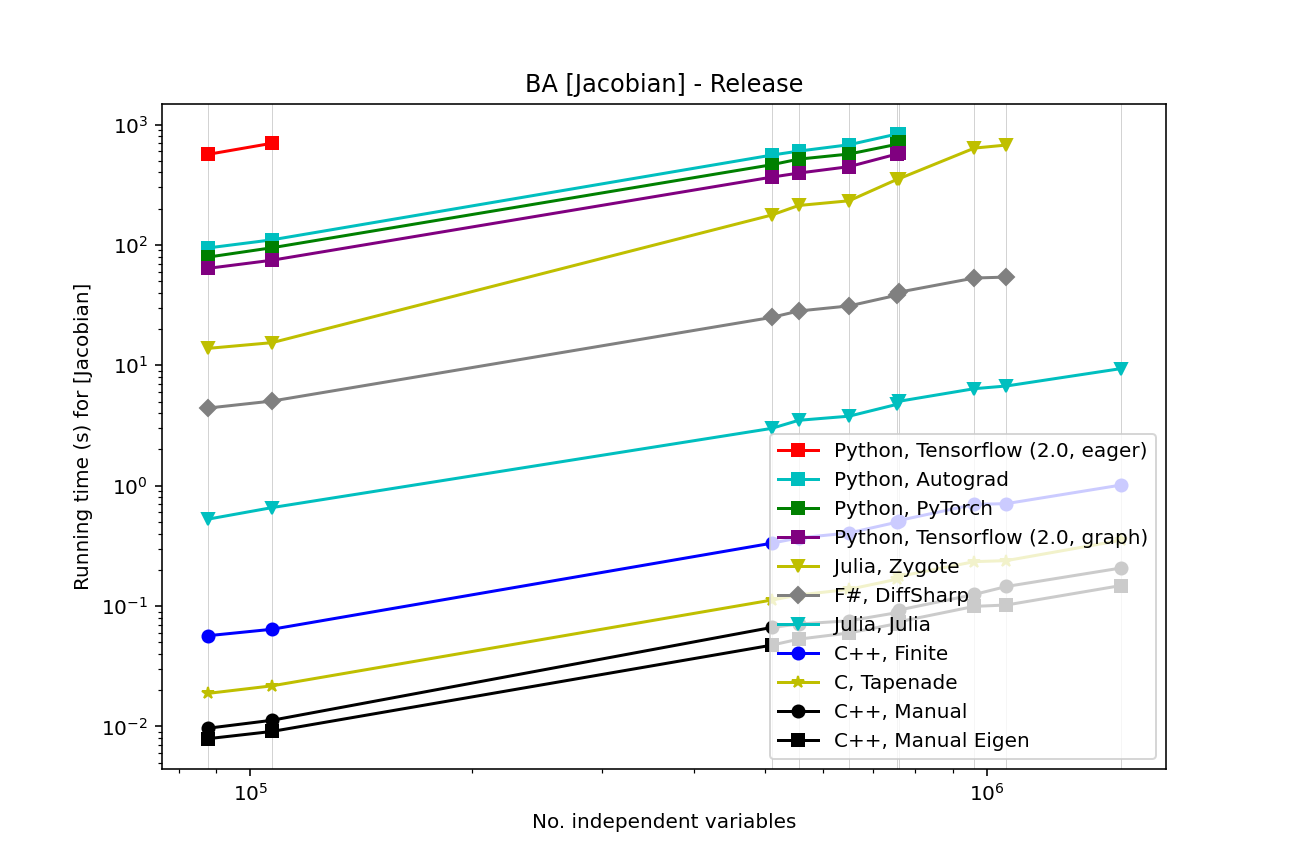
\includegraphics[width=0.5\columnwidth,trim={0 0cm 0 0cm},clip]{ba-jacobian-adbench.png}}
    \caption{The bundle adjustment benchmark which includes Pytorch and Tensorflow (conducted by the ADBench project of microsoft).}\label{bench-ba}
\end{wrapfigure}
Tapenade is $10^{3-5}$ times faster than Pytorch and Tensorflow. However Tapenade is commercial, close sourced and C/Fortran based.
I am pround that NiLang is even better than Tapenade in this benchmark.
I strongly recommend refereees to read the ADBench paper [arXiv:1807.10129], you will be supprise that we choose one of the worlds' best generic AD package as our benchmark target.
We don't benchmark the popular Julia package Flux because it is backended on Zygote, we benchmarked Zygote instead. NiLang is more than one order faster than Zygote in the graph embedding benchmark.

Some referees are wondering if reversible computing are some kind equivalent to tranditonal AD with optimized checkpointing.
I want to emphsis that reversible programming shows advantage in speed and memory comparing with traditional generic AD mainly for one simple reason: \textit{the coding style and reversible thinking matters.}
In NiLang, a programmer does not have the chance to write ``bad'' code just because every allocation is explicit.
In the sparse matrix dot product example in the appendix.
A reversible program has to preallocate a \texttt{branch\_keeper} to store the decisions of branches to enforce reversibility inside the loop.
If a user is writting it in a freestyle, it impossible to avoid stack operations inside the loop, which will slow down the program.
Allocate automatically for a user is even more dangerous in GPU programming.
In the bundle adjustment benchmark,
we can compile the code on GPU to enjoy a ~200x speed up with no more than 10 extra lines of code.
It is very easy for users to completely avoid allocation inside a loop in NiLang.
On the other side, the optimal checkpointing is a well known hard problem. It does not support using reversibility naturally, and a user does not have full control of the allocation.
%One of the referee mention that to handle the backward rule of ``+'' operation, one do not need to store the inputs of an instruction, gradient of both inputs are $1$. There is no need to trace back the state. We haven't put effort in optimizing such operations yet.
%In NiLang, the backward propagation program generally contains $\sim2$ times more instructions than the forward pass. This factor is estimated by considering the backward rule of the multiplication operation. This is a known bottleneck in the field of generic AD.

Some referees want to know from which aspect NiLang is different from a traditional reversible programming language.
For a long time, the reversible programming languages concerns too much about theoretical elegance and ignored the productivity. People tried to implement functional or object oriented reversible languages.
NiLang is special for that it supports many practical elements like arrays, complex numbers, fixed point numbers and logarithmic numbers and being an eDSL so that it can be used directly to accelerate Zygote framework in Julia.

One of the referee is interested to know the limitations of NiLang. We don't think there will be a differentiable program that can not be not be written reversiblly because any program can be made reversible by storing the inputs. The most severe weakness of NiLang is the floating point arithmetic used for computing suffers from the rounding error.
This issue has a systematic solution by mixing fixed point number and logarithmic number, which will be explain in the next update.

Unexpectedly, 2/4 referees think our result can not be reproduced. Condidering both NiLang and the benchmarks are open source on Github, I don't think this result is justified.
I will address other comments like SVD is available in Pytorch and Tensorflow,
comparing reversible programming and the use of reversibility in ML and the bibliography issues in the main text directly. Thanks for your valuable information.

At last, we encourage referees to view this project more from the ``furture'' perspective.
Nowadays, the energy is becoming one of the most deadly bottleneck for machine learning applications.
From a physicist's perspective, we believe that reversible computing is the only correct approach to solve the energy conundrum.
Classical reversible computing has been scilented for $\sim$15 years, NiLang is trying to bridge the new trend machine learning and the reversible computing.
We will try our best to convey this point better in the updated version. As one of the referee said, it is a long overdue.

\end{document}
